\chapter{Simplex theory}

In this section, we present the various definitions connected
to simplex algorithms. We introduce several methods to measure 
the size of a simplex, including the oriented length. 
We present several methods to compute an
initial simplex, that is, the regular simplex used by Spendley et al.,
the axis-by-axis simplex, Pfeffer's simplex and the randomized 
bounds simplex.
%We also present the simplex gradient, which is a forward or a centered 
%difference formula for the gradient of the cost function.
%The core of this section is from \cite{Kelley1999}.

\section{The simplex}

\begin{definition}
(\emph{Simplex})
A \emph{simplex} $S$ in $\RR^n$ is the convex hull of $n+1$ vertices, that is, 
a simplex $S=\{\bv_i\}_{i=1,n+1}$ is defined 
by its $n+1$ vertices $\bv_i \in \RR^n$ for $i=1,n+1$.
\end{definition}

The $j$-th coordinate of the $i$-th vertex $\bv_i\in\RR^n$ is denoted  
by $(\bv_i)_j\in\RR$.

Box extended the Nelder-Mead algorithm to handle bound and non linear constraints \cite{Box1965}.
To be able to manage difficult cases, he uses a \emph{complex} made of $m\geq n+1$ vertices.

\begin{definition}
(\emph{Complex})
A \emph{complex} $S$ in $\RR^n$ is a set of $m\geq n+1$ vertices, that is, 
a simplex $S=\{\bv_i\}_{i=1,m}$ is defined 
by its $m$ vertices $\bv_i \in \RR^n$ for $i=1,m$.
\end{definition}

In this chapter, we will state clearly when the definition and results can only be applied 
to a simplex or to a more general a complex. 
%Indeed, some definitions such as the simplex gradient cannot be extended to a \emph{complex}
%and are only applicable to a \emph{simplex}.

We assume that we are given a cost function $f:\RR^n\rightarrow\RR$.
Each vertex $\bv_i$ is associated with a function value 
\begin{eqnarray}
f_i = f(\bv_i) \textrm{ for } i=1,m.
\end{eqnarray}
For any complex, the vertices can be sorted by increasing function values 
\begin{eqnarray}
\label{simplex-sortedfv}
f_1 \leq f_2 \leq \ldots \leq f_n \leq f_m.
\end{eqnarray}

The sorting order is not precisely defined neither in Spendley's et al paper \cite{Spendley1962}
nor in Nelder and Mead's \cite{citeulike:3009487}. 
In \cite{lagarias:112}, the sorting rules are defined precisely to be able to 
state a theoretical convergence result. In practical implementations, though, the 
ordering rules have no measurable influence.

\section{The size of the complex}
\label{section-simplexsize}

Several methods are available to compute the size of a complex.

In this section, we use  the euclidian norm $\|.\|_2$ 
the defined by 
\begin{eqnarray}
\|\bv\|_2 = \sum_{j=1,n}(v_j)^2.
\end{eqnarray}

\begin{definition}
(\emph{Diameter})
The simplex diameter $diam(S)$ is defined by 
\begin{eqnarray}
\label{simplex-diameter}
diam(S) = \max_{i,j=1,m} \|\bv_i - \bv_j\|_2.
\end{eqnarray}
\end{definition}

In practical implementations, computing the diameter 
requires two nested loops over the 
vertices of the simplex, i.e. requires $m^2$ 
operations. This is why authors generally 
prefer to use lengths which are less expensive 
to compute.

\begin{definition}
(\emph{Oriented length})
The two oriented lengths $\sigma_-(S)$ and 
$\sigma_+(S)$ are defined by 
\begin{eqnarray}
\label{simplex-sigma}
\sigma_+(S) = \max_{i=2,m} \|\bv_i - \bv_1\|_2 
\qquad \textrm { and } \qquad \sigma_-(S) = \min_{i=2,m} \|\bv_i - \bv_1\|_2.
\end{eqnarray}
\end{definition}

\begin{proposition}
The diameter and the maximum oriented length
satisfy the following inequalities 
\begin{eqnarray}
\label{simplex-sigma-diam}
\sigma_+(S) \leq diam(S) \leq 2 \sigma_+(S).
\end{eqnarray}
\end{proposition}

\begin{proof}
We begin by proving that
\begin{eqnarray}
\sigma_+(S) \leq diam(S).
\end{eqnarray}
This is directly implied by the inequality
\begin{eqnarray}
\max_{i=2,m} \|\bv_i - \bv_1\|_2
&\leq& \max_{i=1,m} \|\bv_i - \bv_1\|_2 \\
&\leq& \max_{i,j=1,m} \|\bv_i - \bv_j\|_2,
\end{eqnarray}
which concludes the first part of the proof.
We shall now proove the inequality 
\begin{eqnarray}
\label{eq-simplex-ineqdiam}
diam(S) \leq 2 \sigma_+(S).
\end{eqnarray}
We decompose the difference 
$\bv_i - \bv_j$ into 
\begin{eqnarray}
\bv_i - \bv_j = (\bv_i - \bv_1)+(\bv_1 - \bv_j).
\end{eqnarray}
Hence,
\begin{eqnarray}
\| \bv_i - \bv_j\|_2 \leq \|\bv_i - \bv_1\|_2
+\| \bv_1 - \bv_j\|_2.
\end{eqnarray}
We take the maximum over $i$ and $j$,
which leads to
\begin{eqnarray}
\max_{i,j=1,m}\| \bv_i - \bv_j\|_2 
&\leq& \max_{i=1,m}\|\bv_i - \bv_1\|_2 
+\max_{j=1,m}\| \bv_1 - \bv_j\|_2 \\
&\leq& 2 \max_{i=1,m}\|\bv_i - \bv_1\|_2.
\end{eqnarray}
With the definitions of the diameter
and the oriented length, this immediately 
prooves the inequality 
\ref{eq-simplex-ineqdiam}.
\end{proof}

In Nash's book \cite{nla.cat-vn1060620}, the size of the simplex $s_N(S)$ is measured
based on the 1-norm and is defined by 
\begin{eqnarray}
\label{simplex-sizenash}
s_N(S) = \sum_{i=2,m} \|\bv_i - \bv_1\|_1
\end{eqnarray}
where the 1-norm is defined by 
\begin{eqnarray}
\label{simplex-sizenash2}
\|\bv_i \|_1 = \sum_{j=1,n} |(\bv_i)_j|.
\end{eqnarray}

The \scifunction{optimsimplex\_size} function provides all these size algorithms.
In the following example, we create an axis-by-axis simplex 
with length unity and compute its length by several methods.

\lstset{language=scilabscript}
\begin{lstlisting}
xx0 = [0.0 0.0];
si = optimsimplex_new ( "axes" , x0 );
methodlist = [
"sigmaplus" 
"sigmaminus"
"Nash"
"diameter"
];
for i = 1:size(methodlist,"*")
  m = methodlist ( i );
  ss = optimsimplex_size ( si , m );
  mprintf ( "%s: %f\n", m , ss );
end
optimsimplex_destroy(si)
\end{lstlisting}
The previous script produces the following output.
\lstset{language=scilabscript}
\begin{lstlisting}
sigmaplus: 1.000000
sigmaminus: 1.000000
Nash: 2.000000
diameter: 1.414214
\end{lstlisting}
We check that the diameter is equal to $diam(S) = \sqrt{2}$.
We see that inequality \ref{simplex-sigma-diam} is satisfied since 
$\sigma_+(S)=1\leq \sqrt{2} \leq 2 = 2\sigma_+(S)$.

\section{The initial simplex}

While most of the theory can be developed without being very specific 
about the initial simplex, it plays a very important role in practice.
All approaches are based on the initial guess $\bx_0\in\RR^n$ and create a 
geometric shape based on this point.

In this section, we present the various approach to design the initial 
simplex. In the first part, we emphasize the importance of the initial
simplex in optimization algorithms. Then we present the regular simplex 
by Spendley et al., the axis-by-axis simplex, the randomized bounds approach by Box and 
Pfeffer's simplex.

\subsection{Importance of the initial simplex}

The initial simplex is particularily important in the case of Spendley's et al 
method, where the shape of the simplex is fixed during the iterations.
Therefore, the algorithm can only go through points which are on the pattern
defined by the initial simplex. The pattern presented in figure \ref{fig-nm-simplex-fixedshape}
is typical a fixed-shape simplex algorithm (see \cite{Torczon89multi-directionalsearch}, chapter 3, 
for other patterns of a direct search method).
If, by chance, the pattern is so that the optimum is close to one point 
defined by the pattern, the number of iteration may be small. On the contrary, the 
number of iterations may be large if the pattern does not come close to the 
optimum.

\begin{figure}
\begin{center}
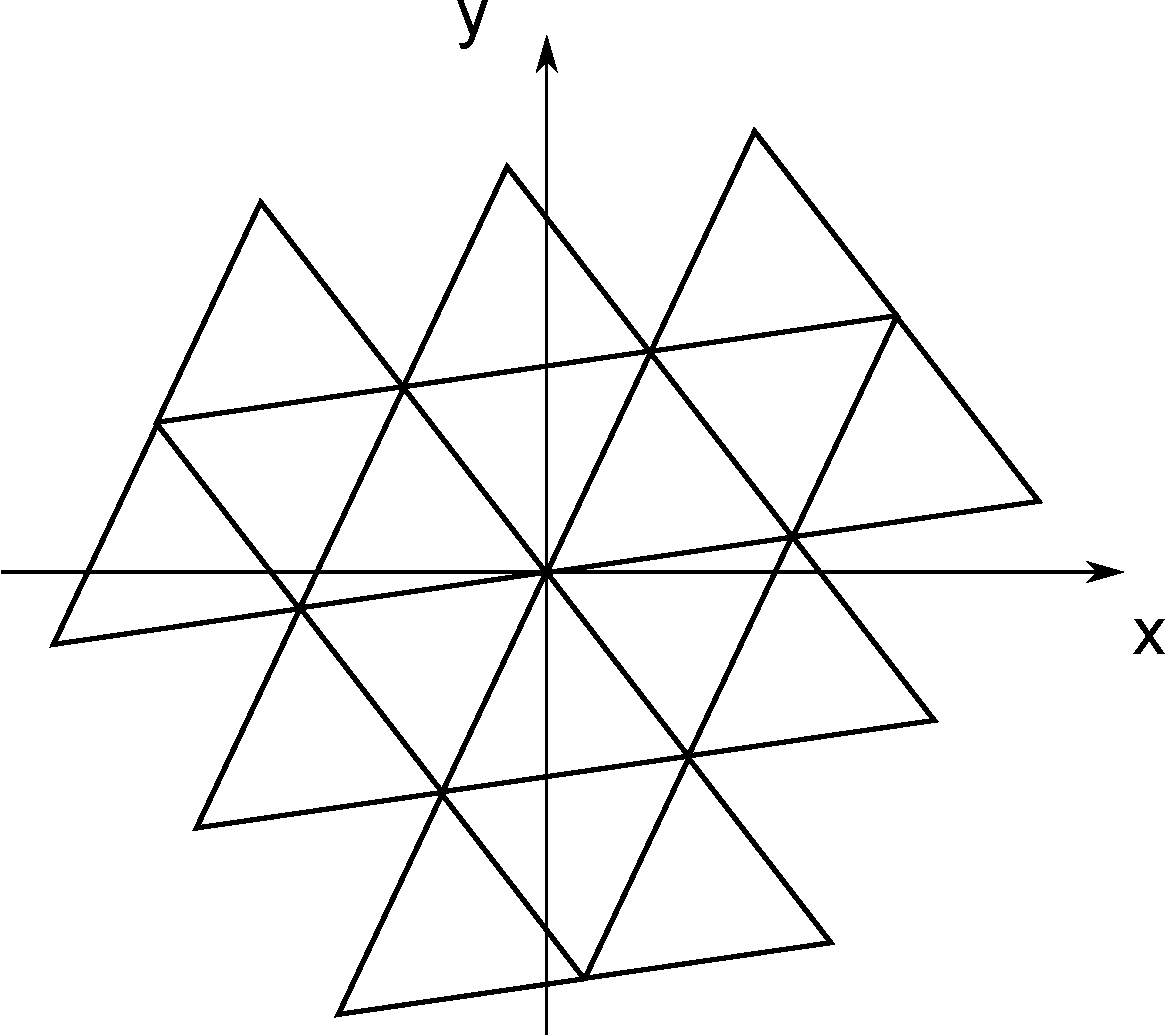
\includegraphics[width=7cm]{simplextheory/simplex_initialfixed.pdf}
\end{center}
\caption{Typical pattern with fixed-shape Spendley's et al algorithm}
\label{fig-nm-simplex-fixedshape}
\end{figure}

The variable-shape simplex algorithm designed by Nelder and Mead is also very
sensitive to the initial simplex.
One of the problems is that the initial simplex should be consistently scaled 
with respect to the unknown $\bx$.
In "An investigation into the efficiency of variants on the simplex method" \cite{parkinson1972}, 
Parkinson and Hutchinson explored 
several improvements of Nelder and Mead's algorithm. First, they investigate the sensitivity
of the algorithm to the initial simplex. Two parameters were investigated,
that is, the initial length and the orientation of the simplex. 
The conclusion of their study with respect to the initial simplex is 
the following. "The orientation of the initial simplex has a significant effect 
on efficiency, but the relationship can be too sensitive for an automatic 
predictor to provide sufficient accuracy at this time."

Since no initial simplex clearly improves on the others, in practice, 
it may be convenient to try different approaches.

\subsection{Spendley's et al regular simplex}
\index{Spendley, W.}
\index{Hext, G. R.}
\index{Himsworth, F. R.}

In their paper \cite{Spendley1962}, Spendley, Hext and Himsworth use a regular 
simplex with given size $\ell>0$. We define the parameters $p,q>0$ as 
\begin{eqnarray}
p &=& \frac{1}{n\sqrt{2}} \left(n-1 + \sqrt{n+1}\right), \\
q &=& \frac{1}{n\sqrt{2}} \left(\sqrt{n+1} - 1\right).
\end{eqnarray}
We can now define the vertices of the simplex $S=\{\bx_i\}_{i=1,n+1}$.
The first vertex of the simplex is the initial guess 
\begin{eqnarray}
\bv_1 &=& \bx_0.
\end{eqnarray}
The other vertices are defined by 
\begin{eqnarray}
(\bv_i)_j &=& 
\left\{
\begin{array}{l}
(\bx_0)_j + \ell p, \textrm{ if } j=i-1,\\
(\bx_0)_j + \ell q, \textrm{ if } j\neq i-1,\\
\end{array}
\right.
\end{eqnarray}
for vertices $i=2,n+1$ and components $j=1,n$, 
where $\ell \in\RR$ is the length of the simplex and satisfies $\ell>0$. Notice that this 
length is the same for all the edges which keeps the simplex regular.

The regular simplex is presented in figure \ref{fig-nm-simplex-regular}.

\begin{figure}
\begin{center}
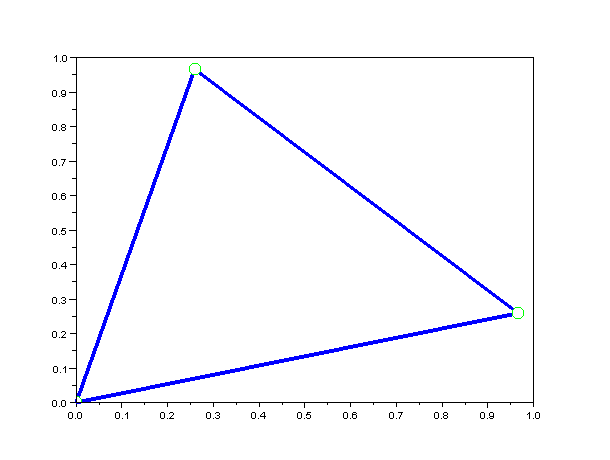
\includegraphics[width=10cm]{simplextheory/simplex_regular.png}
\end{center}
\caption{Regular simplex in 2 dimensions}
\label{fig-nm-simplex-regular}
\end{figure}

In the following Scilab session, we define a regular simplex
with the \scifunction{optimsimplex\_new} function.
\lstset{language=scilabscript}
\begin{lstlisting}
x0 = [0.0 0.0];
si = optimsimplex_new ( "spendley" , x0 );
methodlist = [
"sigmaplus" 
"sigmaminus"
"diameter"
];
for i = 1:size(methodlist,"*")
  m = methodlist ( i );
  ss = optimsimplex_size ( si , m );
  mprintf ( "%s: %f\n", m , ss );
end
optimsimplex_destroy(si);
\end{lstlisting}
The previous script produces the following output.
\lstset{language=scilabscript}
\begin{lstlisting}
sigmaplus: 1.000000
sigmaminus: 1.000000
diameter: 1.000000
\end{lstlisting}
We check that the three sizes $diam(S)$, $\sigma_+(S)$
and $\sigma_-(S)$ are equal, as expected from a regular simplex.

\subsection{Axis-by-axis simplex}

A very efficient and simple approach leads to an axis-by-axis simplex.
This simplex depends on a vector of positive lengths $\bl\in\RR^n$.
The first vertex of the simplex is the initial guess 
\begin{eqnarray}
\bv_1 &=& \bx_0.
\end{eqnarray}
The other vertices are defined by 
\begin{eqnarray}
(\bv_i)_j &=& 
\left\{
\begin{array}{l}
(\bx_0)_j + \ell_j, \textrm{ if } j=i-1,\\
(\bx_0)_j, \textrm{ if } j\neq i-1,\\
\end{array}
\right.
\end{eqnarray}
for vertices $i=2,n+1$ and components $j=1,n$.

This type of simplex is presented in figure \ref{fig-nm-simplex-axes},
where $\ell_1=1$ and $\ell_2=2$.
The axis-by-axis simplex is used in the Nelder-Mead 
algorithm provided in Numerical Recipes in C \cite{NumericalRecipes}.
As stated in \cite{NumericalRecipes}, the length vector $\bl$ can 
be used as a guess for the characteristic length scale of the problem.

\begin{figure}
\begin{center}
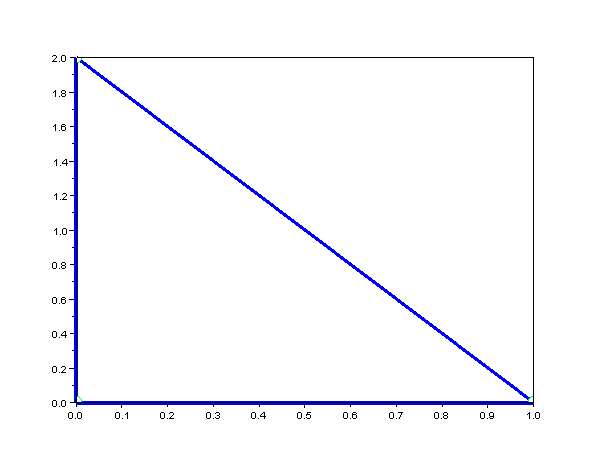
\includegraphics[width=10cm]{simplextheory/simplex_axes.png}
\end{center}
\caption{Axis-based simplex in 2 dimensions -- Notice that the length along the $x$ axis is 1 while the length
along the $y$ axis is 2. }
\label{fig-nm-simplex-axes}
\end{figure}

\subsection{Randomized bounds}

Assume that the variable $\bx\in\RR^n$ is bounded so that 
\begin{eqnarray}
m_j \leq x_j \leq M_j,
\end{eqnarray}
for $j=1,n$, where $m_j,M_j\in\RR$ are minimum 
and maximum bounds and $m_j\leq M_j$.
A method suggested by Box in \cite{Box1965} is 
based on the use of 
pseudo-random numbers. Let 
$\{\theta_{i,j}\}_{i=1,n+1,j=1,n}\in[0,1]$ be 
a sequence of random numbers uniform in the 
interval $[0,1]$.
The first vertex of the simplex is the initial guess 
\begin{eqnarray}
\bv_1 &=& \bx_0.
\end{eqnarray}
The other vertices are defined by 
\begin{eqnarray}
(\bv_i)_j &=& m_j + \theta_{i,j} (M_j - m_j),
\end{eqnarray}
for vertices $i=2,n+1$ and components $j=1,n$.

\subsection{Pfeffer's method}
\index{Pfeffer, L.}

This initial simplex is used in the function \scifunction{fminsearch}
and presented in \cite{Fan2002}. According to \cite{Fan2002}, this simplex is due to L. Pfeffer at Stanford.
The goal of this method is to scale the initial simplex with respect 
to the characteristic lengths of the problem. This allows, for example,
to manage cases where $x_1\approx 1$ and $x_2\approx 10^5$.
As we are going to see, the scaling is defined with respect to the 
initial guess $\bx_0$, with an axis-by-axis method.

The method proceeds by defining $\delta_u,\delta_z>0$, where 
$\delta_u$ is used for usual components of $\bx_0$ and $\delta_z$ is 
used for the case where one component of $\bx_0$ is zero.
The default values for $\delta_u$ and $\delta_z$ are 
\begin{eqnarray}
\delta_u = 0.05 \qquad \textrm{and} \qquad \delta_z = 0.0075.
\end{eqnarray}
The first vertex of the simplex is the initial guess 
\begin{eqnarray}
\bv_1 &=& \bx_0.
\end{eqnarray}
The other vertices are defined by 
\begin{eqnarray}
(\bv_i)_j &=& \left\{
\begin{array}{l}
(\bx_0)_j + \delta_u (\bx_0)_j, \textrm{ if } j=i-1 \textrm{ and } (\bx_0)_{j-1}\neq 0,\\
\delta_z, \textrm{ if } j=i-1 \textrm{ and } (\bx_0)_{j-1}= 0,\\
(\bx_0)_j, \textrm{ if } j\neq i-1,\\
\end{array}
\right.
\end{eqnarray}
for vertices $i=2,n+1$ and components $j=1,n$.

\section{The simplex gradient}
\label{section-simplexgradient}

In this section, we present the simplex gradient and proove 
that this gradient is an approximation of the gradient of the 
objective function, provided that the condition of the matrix 
of simplex directions. We derive the forward 
simplex gradient.

\subsection{Matrix of simplex directions}
\index{matrix of simplex directions}
\index{simplex condition}

We consider here simplices made of $m=n+1$ vertices only.
This allows to define the matrix of simplex directions as presented
in the following definition.

\begin{definition}
(\emph{Matrix of simplex directions})
Assume that $S$ is a set of $m=n+1$ vertices. The $n\times n$ matrix of 
simplex directions $D(S)$ is defined by 
\begin{eqnarray}
D(S) = (\bv_2 - \bv_1 , \bv_2-\bv_1,\ldots,\bv_{n+1} - \bv_1).
\end{eqnarray}
We define by $\{\bd_i\}_{i=1,n}$ the columns of the $n \times n$ matrix $D(S)$,
i.e.
\begin{eqnarray}
D(S)= (\bd_1,\bd_2,\ldots,\bd_n).
\end{eqnarray}
We say that the simplex $S$ is \emph{nonsingular} if the matrix $D(S)$ is \emph{nonsingular}.
We define the \emph{simplex condition} as the $l^2$ condition number 
of the matrix of simplex directions $\kappa(D(S))$.
\end{definition}

The directions $\bd_i$ can be seen as \emph{offsets}, leading from
the first vertex to each vertex $\bv_i$, i.e.
\begin{eqnarray}
\bv_i = \bv_1 + \bd_1, \textrm{ for } i = 1, n.
\end{eqnarray}

\begin{example}
(\emph{A non degenerate simplex})
Consider the axis-by-axis simplex, with first vertex at origin and 
lengths unity. The vertices are defined by 
\begin{eqnarray}
\bv_1=(0,0)^T, \qquad \bv_2=(1,0)^T, \qquad \bv_3=(0,1)^T,
\end{eqnarray}
so that the matrix of simplex directions is 
given by 
\begin{eqnarray}
D = \left(
\begin{array}{cc}
1 & 0 \\
0 & 1 
\end{array}
\right).
\end{eqnarray}
Such a matrix has a unity condition number.

The following Scilab session uses the \scifunction{optimsimplex}
component to generate a axis-by-axis simplex and computes the 
matrix of directions with the \scifunction{optimsimplex\_dirmat}
function.
\lstset{language=scilabscript}
\begin{lstlisting}
x0 = [0.0 0.0];
si = optimsimplex_new ( "axes" , x0 );
D = optimsimplex_dirmat ( si )
k = cond(D)
optimsimplex_destroy(si)
\end{lstlisting}
The previous script produces the following output.
\lstset{language=scilabscript}
\begin{lstlisting}
-->D = optimsimplex_dirmat ( si )
 D  =
    1.    0.  
    0.    1.  
-->k = cond(D)
 k  =
    1.  
\end{lstlisting}
We check that an axis-by-axis simplex has a very low 
condition number.
\end{example}

\begin{example}
(\emph{A degenerate simplex})
In this example, we show that a flat simplex is associated 
with a high condition number.
Consider a flat simplex, defined by its vertices:
\begin{eqnarray}
\bv_1=(0,0)^T, \qquad \bv_2=(1,0)^T, \qquad \bv_3=(1/2,\epsilon)^T,
\end{eqnarray}
with $\epsilon = 10^{-10}$. This simplex is presented in figure \ref{fig-simplex-flat}.

\begin{figure}
\begin{center}
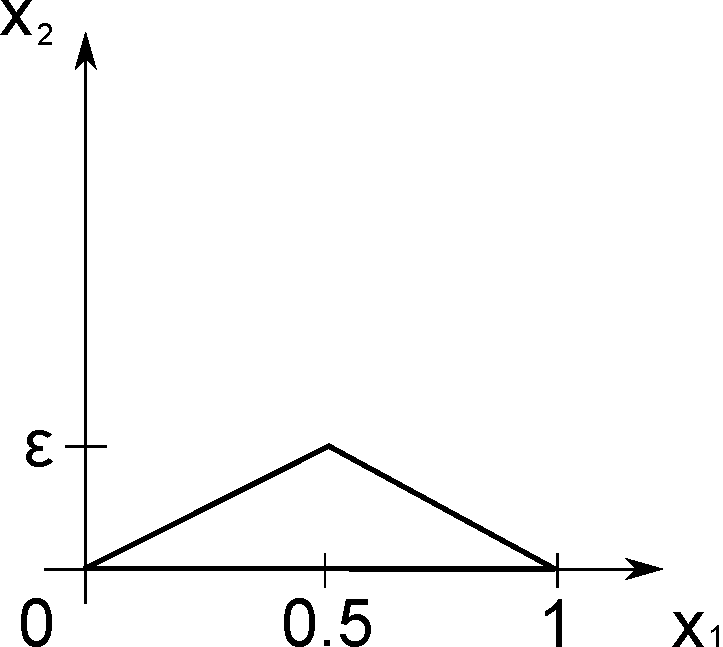
\includegraphics[width=5cm]{simplextheory/simplex_flat.pdf}
\end{center}
\caption{A "flat" simplex in 2 dimensions}
\label{fig-simplex-flat}
\end{figure}

\lstset{language=scilabscript}
\begin{lstlisting}
coords = [
0.0 0.0
1.0 0.0
0.5 1.e-10
];
si = optimsimplex_new ( coords );
D = optimsimplex_dirmat ( si )
k = cond(D)
optimsimplex_destroy(si);
\end{lstlisting}
The previous script produces the following output.
\lstset{language=scilabscript}
\begin{lstlisting}
-->D = optimsimplex_dirmat ( si )
 D  =
    1.    0.5        
    0.    1.000D-10  
-->k = cond(D)
 k  =
    1.250D+10  
\end{lstlisting}
We see that a flat simplex is associated with a high 
condition number. Indeed, a low condition number of the matrix of 
directions is an indication of the non-degeneracy of the simplex.
\end{example}

There is a close relationship between the oriented length
$\sigma_+(S)$ and the $l^2$ norm of the matrix of directions 
$D(S)$ as prooved in the following proposition.

\begin{proposition}
\label{prop-simplex-inequalitysigmaplus}
Let $S$ be a simplex and consider the euclidian norm $\|.\|$.
Therefore,
\begin{eqnarray}
\label{eq-simplex-inequalitysigmaplus}
\|\bd_i\| \leq \sigma_+(S) \leq \|D\|,
\end{eqnarray}
for all $i=1,\ldots,n$.
\end{proposition}

\begin{proof}
It is easy to prove that 
\begin{eqnarray}
\|\bd_i\| \leq \sigma_+(S).
\end{eqnarray}
Indeed, the definition of the oriented length $\sigma_+(S)$
in the case where there are $n+1$ vertices is 
\begin{eqnarray}
\label{eq-simplex-sigma-np1}
\sigma_+(S) &=& \max_{i=2,n+1} \|\bv_i - \bv_1\|_2 \\
& = & \max_{i=1,n} \|\bd_i\|_2,
\end{eqnarray}
which concludes the first part of the proof.

We shall now proove that 
\begin{eqnarray}
\sigma_+(S) \leq \|D\|.
\end{eqnarray}
The euclidian norm is so that (\cite{citeulike:2122238}, section 2.3.1, "Definitions"),
\begin{eqnarray}
\|D \bx\| \leq \|D\| \|\bx\|,
\end{eqnarray}
for any vector $\bx\in\RR^n$. We choose the specific 
vector $\bx$ which has zeros components, except for the $i$-th row,
which is equal to 1, i.e. $\bx=(0,\ldots,0,1,0,\ldots,0)^T$.
With this particular choice of $\bx$ we have the properties $D\bx = \bd_i$
and $\|\bx\| = 1$, so that the previous inequality becomes
\begin{eqnarray}
\label{eq-simplex-normmatrixD1}
\|\bd_i\| \leq \|D\|,
\end{eqnarray}
for all $i=1,\ldots,n$.
We can now take the maximum of the left hand-size of \ref{eq-simplex-normmatrixD1}
and get the oriented length $\sigma_+(S)$, which 
concludes the proof.
\end{proof}

\begin{example}
In the following Scilab session, we define a new simplex 
by its coordinates, so that the matrix of directions 
is not symetric and that the edges do not have unit 
lengths.
\lstset{language=scilabscript}
\begin{lstlisting}
coords = [
0.0 0.0
1.0 0.5
1.0 2.0
];
si = optimsimplex_new ( coords );
D = optimsimplex_dirmat ( si )
for i=1:2
  nd = norm(D(1:2,i),2);
  mprintf( "||d_%d||=%f\n",i,nd)
end
ss = optimsimplex_size ( si , "sigmaplus" );
mprintf( "sigma_+(S)=%f\n",ss);
normmatrix = norm(D);
mprintf( "||D||=%f\n",normmatrix);
optimsimplex_destroy(si);
\end{lstlisting}
The previous script produces the following output.
\lstset{language=scilabscript}
\begin{lstlisting}
||d_1||=1.118034
||d_2||=2.236068
sigma_+(S)=2.236068
||D||=2.422078
\end{lstlisting}
This result is consistent with the inequality \ref{eq-simplex-inequalitysigmaplus}.
\end{example}

\subsection{Taylor's formula}
\label{simplex-Taylor-integral-lipshitz}

The simplex gradient proposition that we shall proove in the 
next section assumes that the gradient $\bg$ of the function $f$ satisfies 
a Lipshitz condition. The following proposition presents 
a result satisfied by such functions.
In order to simplify the notations, we denote by $\|.\|$ the 
euclidian norm.

\begin{proposition}
\label{simplex-prop-taylor-lipshitz}
Assume that $f:\RR^n\rightarrow \RR$ is differentiable and assume that its gradient $\bg$
is defined and continuous. 
Let $\bx\in\RR^n$ be a given point and $\bp\in\RR^n$ a vector.
Assume that the gradient $\bg$ is Lipshitz continuous in a 
neighbourhood of $\bx$ and $\bx+\bp$ with Lipshitz constant
$L$. Then 
\begin{eqnarray}
|f(\bx+\bp) - f(\bx) - \bp^T \bg(\bx) |
&\leq& \frac{1}{2} L \|\bp\|^2.
\end{eqnarray}
\end{proposition}

\begin{proof}
We can write Taylor's expansion of $f$ in a neighbourhood of $\bx$
\begin{eqnarray}
\label{simplex-taylor-gradient}
f(\bx+\bp) &= & f(\bx) + \int_0^1 \bp^T \bg (\bx+t\bp) dt.
\end{eqnarray}
By definition of the Lipshitz condition on $\bg$, we have 
\begin{eqnarray}
\| \bg(\bx) - \bg(\by) \| \leq L \|\bx - \by\|,
\end{eqnarray}
for $\bx$ and $\by$ in that neighbourhood.
Assume that $t\in[0,1]$ and use the particular point $\by = \bx+t\bp$.
We get
\begin{eqnarray}
\label{simplex-lipshitz-gradient}
\| \bg(\bx+t\bp) - \bg(\bx) \| \leq t L \|\bp\|.
\end{eqnarray}
We now use equality \ref{simplex-taylor-gradient}, substract the 
term $\bp^T \bg(\bx)$ and get
\begin{eqnarray}
f(\bx+\bp) - f(\bx) - \bp^T \bg(\bx) = \int_0^1 \bp^T  \left( \bg (\bx+t\bp)  - \bg(\bx) \right) dt.
\end{eqnarray}
Therefore, 
\begin{eqnarray}
\left|f(\bx+\bp) - f(\bx) - \bp^T \bg(\bx) \right|
&=& \left|\int_0^1 \bp^T  \left( \bg (\bx+t\bp)  - \bg(\bx) \right) dt \right|\\
&\leq & \int_0^1 \|\bp\| \left\| \bg (\bx+t\bp)  - \bg(\bx) \right\| dt
\end{eqnarray}
We plug \ref{simplex-lipshitz-gradient} into the previous equality and get
\begin{eqnarray}
\left|f(\bx+\bp) - f(\bx) - \bp^T \bg(\bx) \right| 
&\leq & \int_0^1 L t \|\bp\|^2 dt \\
&\leq& \frac{1}{2} L \|\bp\|^2,
\end{eqnarray}
which concludes the proof.
\end{proof}

\subsection{Forward difference simplex gradient}
\label{simplex-section-forwardgradient}
\index{simplex gradient}

Finite difference formulas are a common tool to compute 
the numerical derivative of a function. In this section, we 
introduce the simplex gradient, which allows to compute 
an approximation of the gradient of the cost function.
As we are going to see, this approximation is more accurate
when the simplex has a low condition number.

We denote by $\delta(S)$ the vector of objective function
differences
\begin{eqnarray}
\delta(S) = ( f(\bv_2) - f(\bv_1), f(\bv_3) - f(\bv_1), \ldots, f(\bv_{n+1}) - f(\bv_1))^T.
\end{eqnarray}
As with classical finite difference formulas, the vector of 
function can be used to compute the simplex gradient.
\begin{definition}
(\emph{Simplex gradient})
Let $S$ be a non singular simplex.  The \emph{simplex gradient} $\overline{\bg}(S)$ is
the unique solution of the linear system of equations 
\begin{eqnarray}
\label{simplex-gradient}
D(S)^T \overline{\bg}(S) = \delta(S).
\end{eqnarray}
\end{definition}

By hypothesis, the simplex $S$ is nonsingular so that the 
linear system of equations has a unique solution, which is 
equal to 
\begin{eqnarray}
\overline{\bg}(S) = (D(S)^T)^{-1} \delta(S).
\end{eqnarray}
By hypothesis, the matrix $D(S)$ is non singular, therefore the transpose of the 
inverse is equal to the inverse of the 
transpose (\cite{citeulike:2122238}, section 2.1.3, "Matrix Inverse"), 
i.e. $(D(S)^T)^{-1} = (D(S)^{-1})^T$.
We denote by $D(S)^{-T}$ the inverse of the transpose so that the previous 
equality becomes 
\begin{eqnarray}
\overline{\bg}(S) = D(S)^{-T} \delta(S).
\end{eqnarray}
In practice, the matrix of simplex direction is not inverted
and the solution of \ref{simplex-gradient} is computed directly, 
using classical linear algebra libraries, like Lapack for example.

The simplex gradient is an approximation of the 
gradient $\bg$ of the function $f$, as presented in the following 
proposition.

\begin{proposition}
Let $S$ be a simplex. Let the gradient $\bg$ be Lipshitz continuous in a neighbourhood
of $S$ with Lipshitz constant $L$. Consider the euclidian norm $\|.\|$. Then, there is $K>0$,
depending only on $L$ such that 
\begin{eqnarray}
\label{eq-inequality-simplexgradient}
\| \bg(\bv_1) - \overline{\bg}(S) \|_2 \leq K \kappa(S) \sigma_+(S).
\end{eqnarray}
\end{proposition}

\begin{proof}
We can write the difference between the simplex 
gradient and the gradient in the following form
\begin{eqnarray}
\overline{\bg}(S) - \bg(\bv_1) = D(S)^{-T} \left( D(S)^T \overline{\bg}(S) - D(S)^T \bg(\bv_1) \right).
\end{eqnarray}
We now plug the simplex gradient definition \ref{simplex-gradient} 
into the previous equality and get
\begin{eqnarray}
\label{eq-simplex-gradient1}
\overline{\bg}(S) - \bg(\bv_1) = D(S)^{-T} \left( \delta(S) - D(S)^T \bg(\bv_1) \right).
\end{eqnarray}

The fact that the euclidian norm $\|.\|$ satisfies the 
inequality 
\begin{eqnarray}
\| A B \| \leq \|A\|\|B\|,
\end{eqnarray}
for any matrices $A$ and $B$ with suitable number of rows 
and columns (\cite{citeulike:2122238}, section 2.3, "Matrix Norms") 
plays an important role in the results that we are going to derive.
Indeed, we can compute the euclidian norm of both sides 
of equation \ref{eq-simplex-gradient1} and get
\begin{eqnarray}
\left\| \overline{\bg}(S) - \bg(\bv_1) \right\| 
&=& \left\| D(S)^{-T} \left( \delta(S) - D(S)^T \bg(\bv_1) \right) \right\|.
\end{eqnarray}
Therefore, 
\begin{eqnarray}
\label{eq-simplex-gradient2}
\left\| \overline{\bg}(S) - \bg(\bv_1) \right\| 
&\leq& \left\| D(S)^{-T} \right\| \left\| \delta(S) - D(S)^T \bg(\bv_1) \right\|.
\end{eqnarray}
The suite of the proof is based on the computation of the right-hand side 
of equation \ref{eq-simplex-gradient2}, that is, the computation of the norm
of the vector $\delta(S) - D(S)^T \bg(\bv_1)$.

By hypothesis, the gradient $\bg$ is Lipshitz continuous in 
a neighbourhood of $S$. By proposition \ref{simplex-prop-taylor-lipshitz},
we have 
\begin{eqnarray}
\left| f(\bv_1 + \bd_i) - f(\bv_1) - \bd_i^T \bg(\bv_1) \right| \leq \frac{1}{2} L \|\bd_i\|^2,
\end{eqnarray}
for $i=1,n$.
By definition of the direction $\bd_i$, we have $\bv_1 + \bd_i = \bv_i$ for 
$i = 1,n$. By proposition \ref{prop-simplex-inequalitysigmaplus},
we have $\|\bd_j\| \leq \sigma_+(S)$ for all $j=1,n$.
Hence, 
\begin{eqnarray}
\label{simplex-eq-taylor-lipshitz1}
\left| f(\bv_i) - f(\bv_1) - \bd_i^T \bg(\bv_1) \right| \leq \frac{1}{2} L \sigma_+(S)^2,
\end{eqnarray}
We can use this to compute the euclidian norm of the 
vector $\delta(S) - D^T \bg(\bv_1)$. Using ineguality \ref{simplex-eq-taylor-lipshitz1},
the square of the norm of this vector is 
\begin{eqnarray}
\left\| \delta(S) - D^T \bg(\bv_1) \right\|^2 
& = & \sum_{i=1,n} \left( f(\bv_i) - f(\bv_1) - \bd_i^T \bg(\bv_1)\right)^2 \\
&\leq & \sum_{i=1,n} \left( \frac{1}{2} L \sigma_+(S)^2 \right)^2\\
&\leq & n \left( \frac{1}{2} L \sigma_+(S)^2 \right)^2
\end{eqnarray}
which finally implies
\begin{eqnarray}
\left\| \delta(S) - D^T \bg(\bv_1) \right\|^2 
\leq \frac{1}{2} \sqrt{n} L \sigma_+(S)^2.
\end{eqnarray}
Let us define the constant $K = \frac{1}{2} \sqrt{n} L$.
The previous inequality becomes
\begin{eqnarray}
\left\| \delta(S) - D^T \bg(\bv_1) \right\|^2 
\leq K \sigma_+(S)^2.
\end{eqnarray}
We can now plug the previous equality into inequality \ref{eq-simplex-gradient2}
and get
\begin{eqnarray}
\left\| \overline{\bg}(S) - \bg(\bv_1) \right\| 
&\leq& K  \left\| D(S)^{-T} \right\| \sigma_+(S)^2.
\end{eqnarray}
By proposition \ref{prop-simplex-inequalitysigmaplus},
we have $\sigma_+(S) \leq \|D\|$, so that the previous inequality
is transformed into
\begin{eqnarray}
\left\| \overline{\bg}(S) - \bg(\bv_1) \right\| 
&\leq& K  \left\| D(S)^{-T} \right\| \left\| D(S) \right\| \sigma_+(S).
\end{eqnarray}
The $l^2$ norm of the matrix $D(S)$ is the largest eigenvalue 
of the matrix $D(S)^T D(S)$, 
so that the norm is not affected by transposition, which implies that
$\left\| D(S)^{-T} \right\| = \left\| D(S)^{-1} \right\|$. 
The condition number of the matrix of direction $\kappa(S)$
is equal to $\left\| D(S)^{-1} \right\| \left\| D(S) \right\|$
(\cite{citeulike:2122238}, section 2.7.2, "Condition"),
which concludes the proof.
\end{proof}

\begin{example}
(\emph{Simplex gradient with a non-degenerate simplex})
In the following Scilab session, we define the 
function $f(\bx)=x_1^2 + x_2^2$, where $\bx\in\RR^2$.
The exact gradient of this function is $\bg=(x_1,x_2)^T$.
We create an axis-by-axis simplex based on the relatively
small length $\ell=10^{-3}$. This simplex defines 
a rectangular triangle, similar to the one presented in
figure \ref{fig-nm-simplex-axes}, but with smaller 
edges.

\lstset{language=scilabscript}
\begin{lstlisting}
function y = myfunction ( x )
  y = x(1)^2 + x(2)^2
endfunction
x0 = [1.0 1.0];
len = 1.e-3;
si = optimsimplex_new ( "axes" , x0 , myfunction , len );
sg = optimsimplex_gradientfv ( si );
mprintf ( "Simplex Gradient=(%f %f)^T\n",sg(1),sg(2));
eg = [2 * x0(1) 2 * x0(2)].';
mprintf ( "Exact Gradient=(%f %f)^T\n",eg(1),eg(2));
err = norm(sg-eg)/norm(eg);
mprintf ( "Relative Error = %e\n",err);
err = norm(sg-eg);
mprintf ( "Absolute Error = %e\n",err);
D = optimsimplex_dirmat ( si );
k = cond(D);
mprintf ( "k(D)=%f\n",k);
ss = optimsimplex_size ( si );
mprintf ( "sigma_+(D)=%e\n",ss);
optimsimplex_destroy(si);
\end{lstlisting}

The previous script produces the following output.
\lstset{language=scilabscript}
\begin{lstlisting}
Simplex Gradient=(2.001000 2.001000)^T
Exact Gradient=(2.000000 2.000000)^T
Absolute Error = 1.414214e-003
k(D)=1.000000
sigma_+(D)=1.000000e-003
\end{lstlisting}
We check that the inequality \ref{eq-inequality-simplexgradient}
gives an accurate measure of the approximation. Indeed, since the 
Lipshitz constant for the gradient $\bg$ is $L=2$,
we have the constant $K=\sqrt{2}$.
\end{example}

\begin{example}
(\emph{Simplex gradient with a simplex close to degenerate})
We consider what happens when an axis-by-axis simplex is transformed into
a degenerate simplex. This situation is presented in figure \ref{fig-simplex-towardflat},
where the third vertex moves on a circle with radius $0.5.10^{-3}$
toward the center of an edge. Therefore the simplex degenerates
and its condition number increases dramatically.

\begin{figure}
\begin{center}
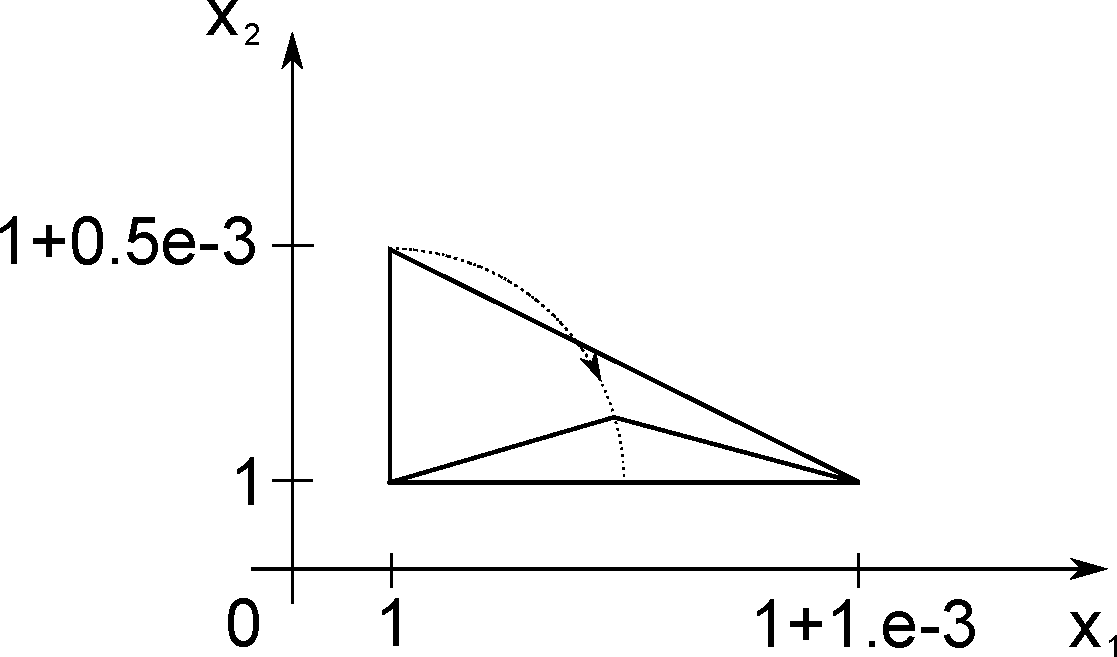
\includegraphics[width=7cm]{simplextheory/simplex_towardflat.pdf}
\end{center}
\caption{An axis-by-axis simplex which degenerates into a "flat" simplex in 2 dimensions.}
\label{fig-simplex-towardflat}
\end{figure}

In the following Scilab script, we create a simplex 
as presented in figure \ref{fig-simplex-towardflat}.
We use decreasing values of the angle $\theta$ between the 
two directions, starting from $\theta=90$~(\degre) and going 
down to $\theta=0.001$~(\degre).
Then we compute the gradient and the absolute error,
as well as the condition number and the size of the simplex.

\lstset{language=scilabscript}
\begin{lstlisting}
R = 0.5e-3
coords = [
  1.0 1.0
  1.0+1.e-3 1.0
];
for theta = [90.0 10.0 1.0 0.1 0.01 0.001]
  C(1,1) = 1.0 + R * cos(theta*%pi/180);
  C(1,2) = 1.0 + R * sin(theta*%pi/180);
  coords(3,1:2) = C;
  si = optimsimplex_new ( coords , myfunction );
  sg = optimsimplex_gradientfv ( si );
  eg = [2 * x0(1) 2 * x0(2)].';
  err = norm(sg-eg);
  D = optimsimplex_dirmat ( si );
  k = cond(D);
  ss = optimsimplex_size ( si );
  mprintf ( "%f %e %e %e\n",theta , ss , err , k);
  optimsimplex_destroy(si);
end
\end{lstlisting}

The results are presented in table \ref{fig-simplex-towardflat-table}.

\begin{figure}
\begin{center}
\begin{tabular}{|l|l|l|l|}
\hline
$\theta$ (\degre) & $\sigma_+(S)$ & $\left\| \overline{\bg}(S) - \bg(\bv_1) \right\|$ & $\kappa(S)$  \\
\hline
90.000000 & 1.000000e-003 & 1.118034e-003 & 2.000000e+000 \\
10.000000 & 1.000000e-003 & 2.965584e-003 & 1.432713e+001 \\
1.000000 & 1.000000e-003 & 2.865807e-002 & 1.432397e+002 \\
0.100000 & 1.000000e-003 & 2.864799e-001 & 1.432395e+003 \\
0.010000 & 1.000000e-003 & 2.864789e+000 & 1.432394e+004 \\
0.001000 & 1.000000e-003 & 2.864789e+001 & 1.432394e+005 \\
\hline
\end{tabular}
\end{center}
\label{fig-simplex-towardflat-table}
\end{figure}
We see that while the oriented length $\sigma_+(S)$ is constant,
the simplex gradient is more and more inaccurate as the 
condition number $\kappa(S)$ is increasing.
\end{example}

\section{References and notes}
\index{Kelley, C. T.}

The section \ref{simplex-section-forwardgradient} and some 
elements of the section \ref{section-simplexsize}
are taken from Kelley's book \cite{Kelley1999}, "Iterative Methods for Optimization".
While this book focus on Nelder-Mead algorithm, Kelley gives a broad
view on optimization and present other algorithms for noisy functions,
like implicit filtering, multidirectional search and the Hooke-Jeeves algorithm.

The section \ref{simplex-Taylor-integral-lipshitz}, which 
present Taylor's formula with a Lisphitz continous gradient is based 
on \cite{numericaloptimization}, "Elements of Analysis, Geometry, Topology",
section "Mean Value Theorem".


